% ═══════════════════════════════════════════════════════════════════════════
\chapter{Resultados}
\label{chap:resultados}
% ═══════════════════════════════════════════════════════════════════════════

El capítulo sigue el orden de las preguntas. La Sección~\ref{sec:especificacion-final} resume cómo se llegó a la especificación final de E3; es la única parte exploratoria del capítulo. Las Secciones~\ref{sec:walkforward} a~\ref{sec:rebote} responden P1 (mejora predictiva), la Sección~\ref{sec:politica} responde P3 (efecto sobre la política), las Secciones~\ref{sec:p2} y~\ref{sec:p2-origen} responden P2 (valor económico), y la Sección~\ref{sec:simulacion} repite ambas evaluaciones en un periodo posterior. Las diferencias de log-verosimilitud se expresan por segundo, sumando las nueve distancias; un valor positivo favorece a E3 tesis.

\section{Especificación final de E3}
\label{sec:especificacion-final}

La especificación se desarrolló dentro del entrenamiento, comparando siempre fuera de muestra por días. Cuatro resultados la definieron.

\paragraph{El estado del mercado explica la mayor parte de la intensidad.} La versión del anteproyecto, $\exp\{g(X)+h(t)\}e^{-k\delta}$ con 44 covariables, redujo a la mitad la log-verosimilitud negativa de Avellaneda--Stoikov en la fase de desarrollo y alcanzó un AUC de 0,84, frente a 0,50 de AS y 0,64--0,65 del Hawkes de una escala. En ablaciones por grupos, el flujo reciente de transacciones fue el más informativo, seguido del libro y de la volatilidad; el OFI resultó casi redundante. El componente horario mejora el lado ask pero no el bid, y se usa solo en el ask. Evaluada después sin reajustar, esa versión superó a AS todos los días de una validación y de dos tests ciegos, aunque uno de los tres veredictos preregistrados no se cumplió (Apéndice~\ref{app:ciegos}).

\paragraph{Gradient boosting frente a random forest (OE3).} Con la misma información, ambos estimadores de $g$ llegan a la misma conclusión: la log-verosimilitud difiere en menos del 1,2\,\% y el AUC en una milésima, en desarrollo y en validación. \textit{Random forest} cuesta entre 4 y 35 veces más tiempo de cómputo, por lo que \textit{gradient boosting} es el estimador principal.

\paragraph{La forma exponencial en la distancia estaba mal calibrada.} A 2~bps, la versión original predecía entre 1,6 y 1,9 veces los cruces observados. Reemplazar $-k\delta$ por la curva monótona \eqref{eq:f-cerrada} reduce el mayor desvío de $\log(O/E)$ entre distancias de 5,6 a 0,4 en el ask y de 8,1 a 2,3 en el bid, con una mejora de $+0{,}031$ y $+0{,}032$ por segundo en todos los días, sin cambio en el AUC. Modular la curva por el estado, $m(X)f(\delta)$, añade $+0{,}011$ a $+0{,}016$. La curva final cae a $f(2)=-1{,}64$ y $f(20)=-8{,}65$ en el ask ($-1{,}68$ y $-10{,}31$ en el bid): más rápido cerca del precio medio y más lento en la cola.

\paragraph{Faltaban covariables de barrido.} Tras un barrido comprador, el cociente estimado $\lambda_a/\lambda_b$ a 2~bps pasa de 1,3 a 5,6, de modo que E3 capta el impulso del barrido. Pero subestimaba el rebote del lado contrario: tras barridos vendedores llegaban cerca de un 60\,\% más compradores de los esperados. Cinco covariables causales (recorrido firmado, volumen y tiempo desde el último barrido; spread máximo y variación del precio medio en el último segundo) reducen esa brecha de 0,454 a 0,091.

La especificación final, \textbf{E3 tesis}, es \eqref{eq:fkx} con 49 covariables, $h$ horaria en el ask, curva $f$ monótona y $m(X)=\exp(b^\top z)$ con cuatro covariables. Sus coeficientes de modulación son pequeños ($|b_j|\le0{,}10$).


\section{P1: comparación con referencias reforzadas}
\label{sec:walkforward}

Las referencias reciben las mismas mejoras aplicables que E3 (Tabla~\ref{tab:modelos}). El Hawkes de dos escalas ajustado con todo el entrenamiento elige memorias de 1~s y 3,3~ms ($\beta=1$ y $300$~s$^{-1}$) con radio espectral 0,74; el de una escala elige solo la escala rápida.

La Tabla~\ref{tab:wf} y la Figura~\ref{fig:wf-parte} resumen los 34 días fuera de muestra del \textit{walk-forward}. La ventana 1 reproduce exactamente los resultados obtenidos antes con el mismo ajuste (diferencia relativa nula), lo que verifica el código.

\begin{table}[htbp]
\centering\footnotesize
\caption{\textit{Walk-forward} (cinco ventanas semanales, 34 días fuera de muestra; ajuste original). Parte de la mejora de E3 tesis sobre AS base que recupera cada modelo, ventaja de E3 tesis por intervalo [IC95 por días] y AUC a $\delta=2$~bps.}
\label{tab:wf}
\resizebox{\textwidth}{!}{%
\begin{tabular}{@{}lrrccrr@{}}\toprule
& \multicolumn{2}{c}{Parte de la mejora} & \multicolumn{2}{c}{E3 tesis $-$ modelo} & \multicolumn{2}{c}{AUC}\\
\cmidrule(lr){2-3}\cmidrule(lr){4-5}\cmidrule(l){6-7}
Modelo & ask & bid & ask & bid & ask & bid\\\midrule
\textbf{E3 tesis} & 100\,\% & 100\,\% & -- & -- & 0,834 & 0,825\\
E3-fkX (44 cov.) & 98,6\,\% & 99,5\,\% & $+0{,}024$ [0,005; 0,050] & $+0{,}008$ [0,002; 0,015] & 0,833 & 0,824\\
E3 base & 92,7\,\% & 93,5\,\% & $+0{,}127$ [0,058; 0,225] & $+0{,}110$ [0,045; 0,213] & 0,834 & 0,824\\
GLM lineal (49 cov.) & 90,9\,\% & 90,1\,\% & $+0{,}158$ [0,111; 0,223] & $+0{,}166$ [0,102; 0,254] & 0,821 & 0,814\\
Hawkes 2 esc. + S & 79,1\,\% & 75,8\,\% & $+0{,}365$ [0,275; 0,470] & $+0{,}408$ [0,286; 0,554] & 0,780 & 0,772\\
Hawkes 2 esc. + h + f & 61,7\,\% & 60,9\,\% & $+0{,}668$ [0,442; 0,962] & $+0{,}659$ [0,424; 0,959] & 0,757 & 0,752\\
Hawkes 1 esc. + S & 52,4\,\% & 49,0\,\% & $+0{,}830$ [0,593; 1,114] & $+0{,}860$ [0,565; 1,206] & 0,731 & 0,725\\
AS + S & 50,8\,\% & 47,0\,\% & $+0{,}857$ [0,609; 1,152] & $+0{,}893$ [0,582; 1,261] & 0,728 & 0,721\\
Hawkes 1 esc. + h + f & 9,2\,\% & 9,1\,\% & $+1{,}582$ [0,995; 2,303] & $+1{,}530$ [0,941; 2,240] & 0,628 & 0,626\\
AS + h + f & 7,4\,\% & 6,9\,\% & $+1{,}614$ [1,012; 2,352] & $+1{,}567$ [0,961; 2,294] & 0,616 & 0,612\\
AS base & 0\,\% & 0\,\% & $+1{,}743$ [1,122; 2,483] & $+1{,}684$ [1,061; 2,440] & 0,500 & 0,500\\\bottomrule
\end{tabular}}
\end{table}

\begin{figure}[htbp]
\centering
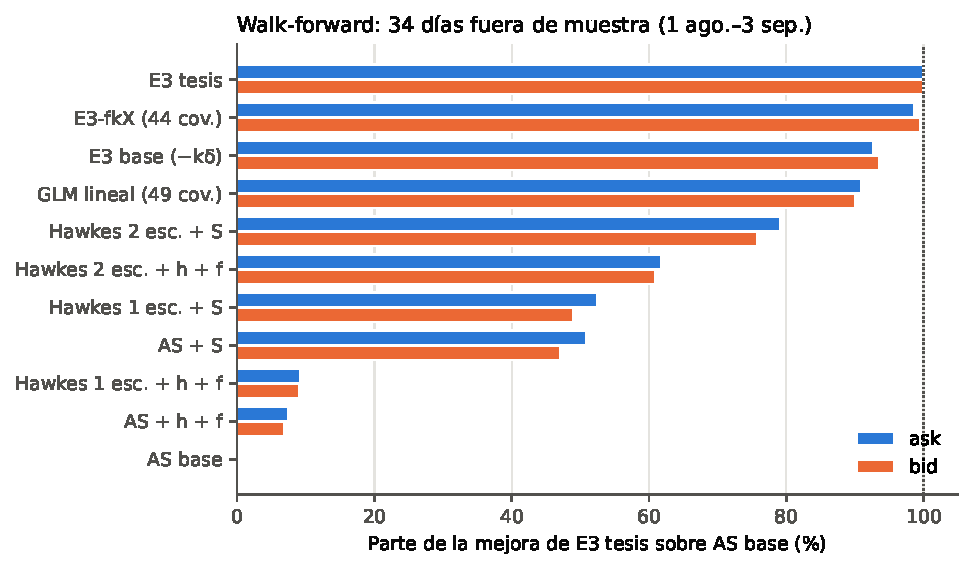
\includegraphics[width=.86\textwidth]{F1_parte_mejora_wf.pdf}
\caption{Parte de la mejora de E3 tesis sobre AS base que recupera cada modelo en el \textit{walk-forward}.}
\label{fig:wf-parte}
\end{figure}

Se cumplen los dos criterios principales del protocolo. \emph{Estabilidad}: E3 tesis supera a cada uno de los diez modelos en las cinco ventanas y en ambos lados (Figura~\ref{fig:wf-ventanas}). \emph{Diferencia global}: el intervalo de confianza de la ventaja es positivo frente a todos; frente a E3-fkX gana 25 y 23 de 34 días, y frente a los demás, 33 o 34 de 34. La ventaja crece en las semanas agitadas (15--28 de agosto), en las que una intensidad constante falla más.

\begin{figure}[htbp]
\centering
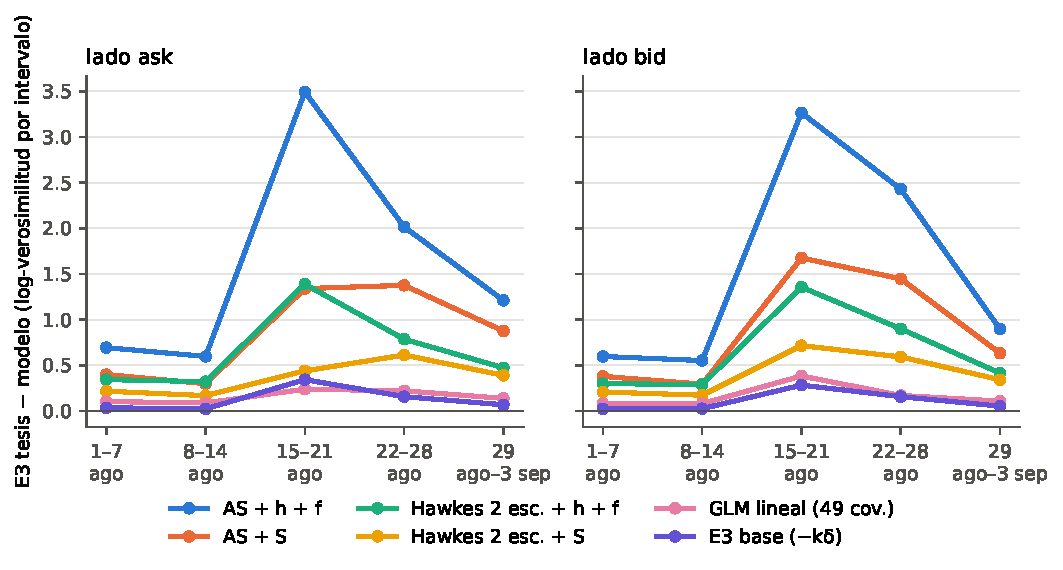
\includegraphics[width=.95\textwidth]{F2_ventaja_por_ventana.pdf}
\caption{Ventaja de E3 tesis sobre seis referencias en cada ventana del \textit{walk-forward}. Todas las curvas quedan por encima de cero.}
\label{fig:wf-ventanas}
\end{figure}

El diagnóstico de sobreajuste compara la ventaja de E3 sobre el GLM lineal en la semana siguiente con la de la última semana ajustada. El cociente está por debajo de 0,5 en dos de cinco ventanas (V4 y V5), en las que la semana ajustada incluye el periodo agitado del 15 al 28 de agosto y la ventaja dentro de muestra se infla; el umbral del protocolo (tres ventanas) no se alcanza. En la ventana 3 el cociente supera 2, porque la semana evaluada es la agitada.

Tres lecturas se desprenden de la Tabla~\ref{tab:wf}. Primera, el estado del libro explica la mayor parte de la mejora: el GLM lineal con las mismas covariables recupera el 90--91\,\%. La no linealidad de $g$ aporta el resto, mejora la discriminación (AUC 0,834 frente a 0,821) y, entre los modelos evaluados, es la que mejor corrige el rebote (Sección~\ref{sec:rebote}). Segunda, la memoria importa, pero con la escala correcta: el Hawkes de dos escalas recupera el 61--62\,\% frente al 9\,\% del de una escala. Tercera, las variables de barrido aportan poco a la verosimilitud global (E3-fkX recupera el 98,6--99,5\,\%), porque los barridos son eventos raros; su valor está en la calibración tras esos eventos.


\section{P1: test final}
\label{sec:test}

Con los once modelos ajustados en todo el entrenamiento y congelados antes de leer el test, se evaluaron una sola vez en el test del 4 al 20 de septiembre, un periodo ya consultado con la versión original de E3. Se cumplen los cuatro criterios preregistrados (Tabla~\ref{tab:test}):
\begin{itemize}[nosep]
\item \textbf{jerarquía}: E3 tesis supera a AS + h + f, AS + S, GLM lineal, Hawkes 2 escalas + h + f y Hawkes 2 escalas + S con IC95 positivo en ambos lados;
\item \textbf{consistencia}: gana 17 de 17 días al Hawkes de dos escalas con señales en ambos lados;
\item \textbf{discriminación}: AUC de 0,813 en ambos lados, por encima de 0,80;
\item \textbf{rebote}: brecha de $+0{,}116$ tras barridos vendedores y $-0{,}139$ tras compradores, dentro de $\pm0{,}15$.
\end{itemize}

\begin{table}[htbp]
\centering\footnotesize
\caption{Test final (4--20 sep., 17 días; modelos congelados con el ajuste corregido, idéntico al original a tres decimales). Parte de la mejora sobre AS base, ventaja de E3 tesis por intervalo [IC95 por días] y días en que gana E3 tesis (ask / bid).}
\label{tab:test}
\resizebox{\textwidth}{!}{%
\begin{tabular}{@{}lrrccc@{}}\toprule
& \multicolumn{2}{c}{Parte de la mejora} & \multicolumn{2}{c}{E3 tesis $-$ modelo} & \\
\cmidrule(lr){2-3}\cmidrule(lr){4-5}
Modelo & ask & bid & ask & bid & Días\\\midrule
E3-fkX (44 cov.) & 99,8\,\% & 98,9\,\% & $+0{,}002$ [$-0{,}004$; 0,008] & $+0{,}015$ [0,003; 0,029] & 10 / 13\\
E3 base & 96,0\,\% & 93,5\,\% & $+0{,}053$ [0,034; 0,073] & $+0{,}087$ [0,047; 0,134] & 16 / 17\\
GLM lineal (49 cov.) & 91,6\,\% & 89,6\,\% & $+0{,}110$ [0,077; 0,145] & $+0{,}140$ [0,089; 0,193] & 16 / 16\\
Hawkes 2 esc. + S & 73,8\,\% & 73,7\,\% & $+0{,}345$ [0,251; 0,454] & $+0{,}353$ [0,263; 0,457] & 17 / 17\\
Hawkes 2 esc. + h + f & 60,3\,\% & 62,3\,\% & $+0{,}523$ [0,377; 0,692] & $+0{,}505$ [0,355; 0,681] & 17 / 17\\
Hawkes 1 esc. + S & 45,1\,\% & 44,6\,\% & $+0{,}723$ [0,494; 0,985] & $+0{,}742$ [0,510; 1,007] & 17 / 17\\
AS + S & 43,6\,\% & 43,0\,\% & $+0{,}742$ [0,508; 1,010] & $+0{,}764$ [0,526; 1,036] & 17 / 17\\
Hawkes 1 esc. + h + f & 11,1\,\% & 12,3\,\% & $+1{,}170$ [0,775; 1,644] & $+1{,}175$ [0,743; 1,678] & 17 / 17\\
AS + h + f & 9,5\,\% & 10,4\,\% & $+1{,}191$ [0,788; 1,671] & $+1{,}200$ [0,759; 1,714] & 17 / 17\\
AS base & 0\,\% & 0\,\% & $+1{,}316$ [0,880; 1,810] & $+1{,}340$ [0,835; 1,953] & 17 / 17\\\bottomrule
\end{tabular}}
\end{table}

El orden de los modelos es el mismo que en el \textit{walk-forward} (Figura~\ref{fig:test-parte}) y el AUC baja de 0,83 a 0,81, una degradación moderada en datos nuevos. Frente a E3-fkX, la ventaja en el lado ask no es significativa: las variables de barrido no mejoran la predicción global en ese lado, aunque sí la calibración del rebote. Los AUC de las referencias en el test son 0,80 (GLM), 0,76--0,77 (Hawkes 2 escalas + S), 0,74--0,75 (Hawkes 2 escalas + h + f), 0,71--0,72 (AS + S), 0,61--0,63 (AS y Hawkes 1 escala con h y f) y 0,50 (AS base).

\begin{figure}[htbp]
\centering
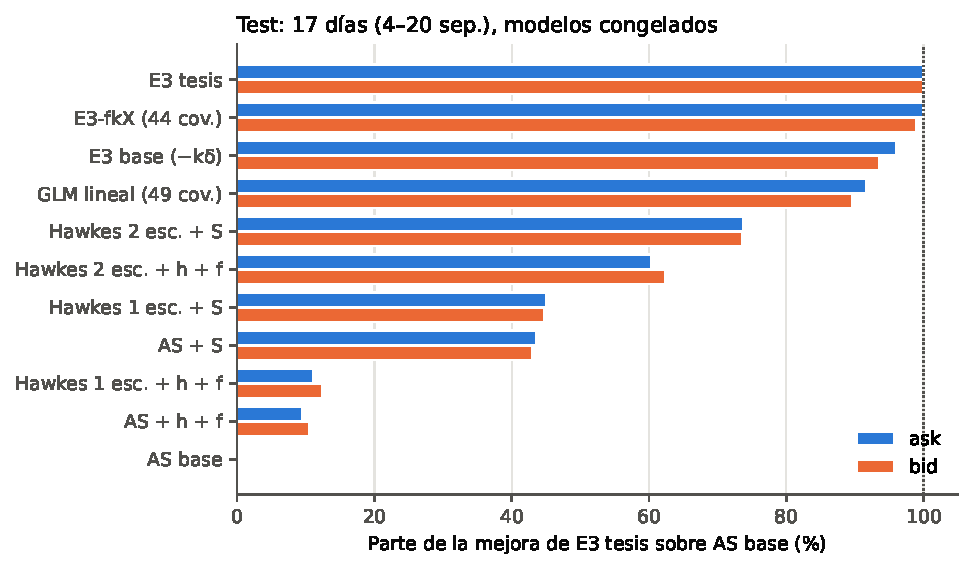
\includegraphics[width=.86\textwidth]{F4_parte_mejora_test.pdf}
\caption{Parte de la mejora de E3 tesis sobre AS base que recupera cada modelo en el test final.}
\label{fig:test-parte}
\end{figure}


\section{P1: calibración tras barridos}
\label{sec:rebote}

La Figura~\ref{fig:rebote} muestra, para el \textit{walk-forward}, la brecha entre la razón O/E del lado contrario tras barridos y la razón O/E habitual, separada por el lado del barrido y por la tendencia de la última hora. Cero indica que el modelo acierta tras un barrido tan bien como en momentos normales.

\begin{figure}[htbp]
\centering
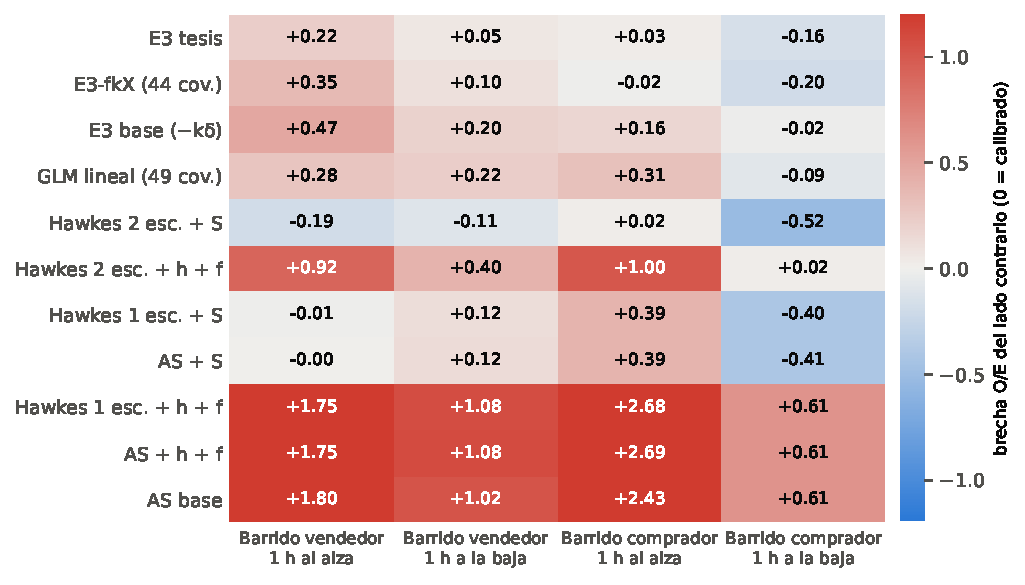
\includegraphics[width=.86\textwidth]{F3_rebote.pdf}
\caption{Brecha del rebote tras barridos en el \textit{walk-forward}, por modelo y situación. Rojo: llegan más agresores del lado contrario de los que el modelo espera; azul: menos.}
\label{fig:rebote}
\end{figure}

Los modelos sin covariables de estado (AS y Hawkes con h y f) subestiman fuertemente el rebote, con brechas de $+0{,}6$ a $+2{,}7$. Las señales lineales lo sobrecorrigen en la celda ``comprador con tendencia bajista'' ($-0{,}4$ a $-0{,}5$). E3 tesis tiene las brechas más cercanas a cero en tres de las cuatro celdas. La celda ``comprador con tendencia bajista'' ($-0{,}16$) no la corrige ningún modelo y queda como limitación declarada. En el test, la celda más débil de E3 tesis es ``comprador con tendencia alcista'' ($-0{,}235$).


\section{P3: política óptima con intensidades estimadas}
\label{sec:politica}

La HJB \eqref{eq:hjb-theta} se resolvió numéricamente con un esquema de Euler implícito linealizado, incondicionalmente estable porque la matriz del sistema es una M-matriz, seguido de un paso de Newton sobre el régimen ergódico. El Hamiltoniano se calcula con la curva de distancia de cada modelo interpolada: $\log\Lambda_i(\delta)$ es lineal a trozos entre los nueve nodos de $\delta$ y se extiende con la pendiente del primer y del último tramo; en cada tramo el máximo de $\Lambda_i(\delta)(1-e^{-\gamma(\delta-p)})/\gamma$ tiene forma cerrada, y $H_i$ es el máximo sobre los tramos, con $\delta$ restringida a $[-5;40]$~bps. Para aplicarla cada segundo se precalculan tablas en $(\ln\sigma^2/A_a,\ln A_b/A_a)$ y, para E3 tesis y E3-fkX, también en $(m_a,m_b)$, con rangos tomados de seis días de entrenamiento. Antes de usarla en el test se verificó en el entrenamiento que:
\begin{itemize}[nosep]
\item con forma exponencial reproduce la solución de la Sección~\ref{sec:hjb-teoria} (diferencia máxima $10^{-14}$), que a su vez reproduce la solución lineal de \citet{Gueant2017};
\item el máximo por tramos coincide con una búsqueda exhaustiva en una rejilla fina (error relativo máximo $2\times10^{-8}$);
\item las distancias son monótonas en el inventario;
\item las tablas reproducen la solución exacta con un error p99 de a lo sumo 0,027~bps en todo $|q|\le10$.
\end{itemize}
Ninguna pendiente de tramo resultó menor que 0,16~bps$^{-1}$ y ninguna distancia óptima tocó los bordes del intervalo. La aversión $\gamma=0{,}01$ se eligió en la fase de desarrollo. La Tabla~\ref{tab:hjb} muestra cómo cambia la política con cada intensidad.

\begin{table}[htbp]
\centering\small
\caption{Distancia óptima en el ask con inventario nulo (bps), mediana en el test; $\gamma=0{,}01$, ajuste corregido. La HJB usa la curva de distancia interpolada; GLFT, una exponencial local.}
\label{tab:hjb}
\begin{tabular}{@{}lcc@{}}\toprule
Intensidad & HJB & GLFT\\\midrule
AS base (forma exponencial) & 1,55 & 1,49\\
E3 base (forma exponencial) & 1,50 & 1,51\\
AS, Hawkes y GLM con curva $f(\delta)$ & 1,11--1,14 & 1,48--1,49\\
E3 tesis & 0,85 & 1,25\\\bottomrule
\end{tabular}
\end{table}

Tres resultados responden a P3. Primero, en GLFT la distancia base no depende del nivel $A$, de modo que las referencias apenas mueven las cotizaciones respecto de AS. Segundo, la forma de la curva sí importa en la solución numérica: con la curva interpolada, los modelos con $f(\delta)$ cotizan unos 0,4~bps más cerca que con una exponencial, y E3 tesis, cuya pendiente cerca del precio medio depende del estado, unos 0,7~bps más cerca. Frente a la versión que aproxima cada intensidad por una exponencial local, el precio cotizado cambia en el 86--99\,\% de las decisiones de esos modelos. Tercero, el cociente $A_b/A_a$ que predice E3 sesga la política hacia un lado incluso con inventario nulo. Los valores negativos de la distancia, que cruzarían el precio medio, se acotan al mejor precio para mantener la orden pasiva.

\section{Valor económico en el test}
\label{sec:p2}
La Tabla~\ref{tab:pnl} y la Figura~\ref{fig:pnl} muestran el desempeño en el test de las tres políticas con las intensidades de los modelos del ajuste corregido, todas con el mismo simulador, la misma orden de 0,01~BTC y el mismo límite de inventario. El precio medio de BTC en el test fue de unos 78\,000~USDT, de modo que cada orden vale unos 780~USDT.

\begin{table}[htbp]
\centering\footnotesize
\caption{PnL de market making en el test (17 días), bruto de comisiones; ajuste corregido. HJB con curva de distancia interpolada; GLFT con exponencial local. PnL por ejecución con IC95 por días.}
\label{tab:pnl}
\setlength{\tabcolsep}{3.5pt}
\resizebox{\textwidth}{!}{%
\begin{tabular}{@{}llrrcr@{}}\toprule
Política & Intensidad & Ejec./día & PnL/día (USDT) & PnL por ejec. (bps) & Días $>0$\\\midrule
\multirow{4}{*}{Miope} & E3 tesis & 4\,222 & $-443$ & $-1{,}34$ [$-1{,}48$; $-1{,}19$] & 0/17\\
 & AS, Hawkes, GLM con $f(\delta)$ & 3\,806 & $-385$ & $-1{,}29$ [$-1{,}45$; $-1{,}14$] & 0/17\\
 & AS base y E3 base ($\delta=2$) & 1\,173 & $-121$ & $-1{,}32$ [$-1{,}84$; $-0{,}78$] & 4/17\\
 & $\delta$ fijo 0,5~bps & 6\,872 & $-720$ & $-1{,}34$ [$-1{,}42$; $-1{,}24$] & 0/17\\\midrule
\multirow{6}{*}{HJB} & E3 tesis & 2\,451 & $-253$ & $-1{,}32$ [$-1{,}42$; $-1{,}20$] & 0/17\\
 & E3 base & 1\,677 & $-175$ & $-1{,}34$ [$-1{,}51$; $-1{,}15$] & 0/17\\
 & GLM lineal & 2\,549 & $-262$ & $-1{,}32$ [$-1{,}40$; $-1{,}22$] & 0/17\\
 & Hawkes 2 esc. + S & 3\,543 & $-355$ & $-1{,}28$ [$-1{,}35$; $-1{,}18$] & 0/17\\
 & AS + h + f & 3\,982 & $-398$ & $-1{,}28$ [$-1{,}35$; $-1{,}18$] & 0/17\\
 & AS base & 2\,218 & $-219$ & $-1{,}26$ [$-1{,}37$; $-1{,}14$] & 0/17\\\midrule
\multirow{3}{*}{GLFT} & E3 tesis & 3\,008 & $-289$ & $-1{,}23$ [$-1{,}32$; $-1{,}11$] & 0/17\\
 & Hawkes 2 esc. + S & 2\,321 & $-228$ & $-1{,}25$ [$-1{,}36$; $-1{,}12$] & 0/17\\
 & AS base & 2\,223 & $-218$ & $-1{,}25$ [$-1{,}35$; $-1{,}13$] & 0/17\\\bottomrule
\end{tabular}}
\end{table}

\begin{figure}[htbp]
\centering
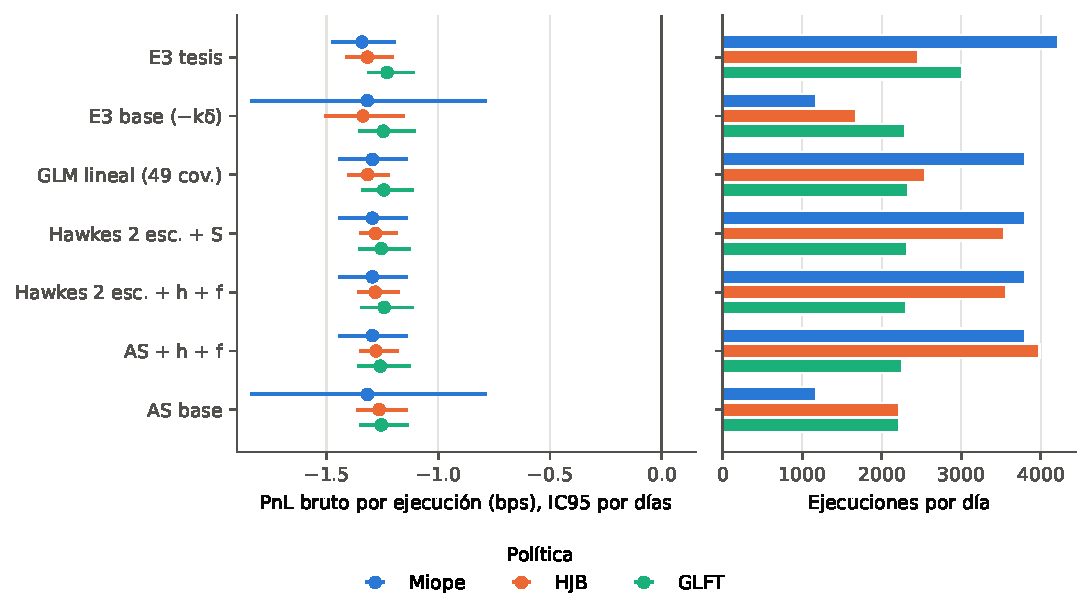
\includegraphics[width=.98\textwidth]{F5_pnl_test.pdf}
\caption{PnL bruto por ejecución (izquierda, IC95 por días) y ejecuciones por día (derecha) en el test, por intensidad y política; ajuste corregido, HJB con curva interpolada.}
\label{fig:pnl}
\end{figure}

\begin{itemize}[nosep]
\item \textbf{Las diferencias por ejecución entre combinaciones no son concluyentes.} Todas pierden entre $-1{,}22$ y $-1{,}34$~bps antes de comisiones, y las diferencias pareadas entre E3 tesis y cada referencia, en las tres políticas, tienen intervalos que incluyen el cero.
\item \textbf{E3 cambia la política, no el resultado por ejecución.} Con la HJB, E3 tesis opera entre un 31 y un 38\,\% menos que AS y Hawkes con la misma forma de curva (2\,451 frente a 3\,543--3\,982 ejecuciones por día) y pierde menos por día ($-253$ frente a $-355$ a $-398$~USDT); frente a AS base, con forma exponencial, opera un 10\,\% más. La pérdida por ejecución es similar en todos los casos.
\item \textbf{La curva interpolada cambia las cotizaciones, no la pérdida por ejecución.} Frente a la HJB con exponencial local, aumenta las ejecuciones entre 723 y 1\,735 por día según el modelo, con diferencias en el PnL por ejecución de $-0{,}04$ a $+0{,}02$~bps, todas con intervalos que incluyen el cero.
\item \textbf{La regla miope colapsa a distancias fijas.} Como solo usa la forma de $\lambda$ en $\delta$, los modelos con curva $f(\delta)$ fija eligen siempre 1~bps y los de forma exponencial siempre 2~bps; solo E3 tesis varía la distancia con el estado.
\item \textbf{Las comisiones agravan el resultado.} Con la comisión maker estándar de un participante minorista (7,5--10~bps por ejecución), todas las combinaciones pierden entre 9 y 11~bps por ejecución.
\end{itemize}

\section{Simulación del 21 de septiembre al 26 de octubre}
\label{sec:simulacion}

Con los mismos modelos y políticas, sin ningún reajuste, se evaluaron los 36 días posteriores al test. Antes de abrir el periodo se comprobó que el código reproduce exactamente un día del test (diferencia nula en predicción, ejecuciones y PnL).

\begin{table}[htbp]
\centering\footnotesize
\caption{Simulación (21 sep.--26 oct., 36 días; modelos congelados). Parte de la mejora sobre AS base, ventaja de E3 tesis por segundo [IC95 por días], días ganados y AUC (ask / bid).}
\label{tab:sim}
\resizebox{\textwidth}{!}{%
\begin{tabular}{@{}lrrcccc@{}}\toprule
& \multicolumn{2}{c}{Parte de la mejora} & \multicolumn{2}{c}{E3 tesis $-$ modelo} & & \\
\cmidrule(lr){2-3}\cmidrule(lr){4-5}
Modelo & ask & bid & ask & bid & Días & AUC\\\midrule
\textbf{E3 tesis} & 100\,\% & 100\,\% & -- & -- & -- & 0,848 / 0,842\\
E3-fkX (44 cov.) & 100,2\,\% & 99,3\,\% & $-0{,}003$ [$-0{,}010$; 0,005] & $+0{,}008$ [0,003; 0,014] & 16 / 28 & 0,848 / 0,842\\
E3 base & 94,5\,\% & 94,2\,\% & $+0{,}065$ [0,047; 0,085] & $+0{,}074$ [0,058; 0,092] & 33 / 36 & 0,847 / 0,842\\
GLM lineal (49 cov.) & 90,8\,\% & 90,0\,\% & $+0{,}107$ [0,071; 0,146] & $+0{,}129$ [0,077; 0,177] & 32 / 35 & 0,840 / 0,836\\
Hawkes 2 esc. + S & 70,2\,\% & 70,7\,\% & $+0{,}347$ [0,295; 0,406] & $+0{,}376$ [0,321; 0,441] & 36 / 36 & 0,785 / 0,783\\
Hawkes 2 esc. + h + f & 58,8\,\% & 62,2\,\% & $+0{,}479$ [0,389; 0,584] & $+0{,}486$ [0,403; 0,582] & 36 / 36 & 0,764 / 0,765\\
Hawkes 1 esc. + S & 43,6\,\% & 41,9\,\% & $+0{,}657$ [0,551; 0,770] & $+0{,}747$ [0,613; 0,892] & 36 / 36 & 0,746 / 0,743\\
AS + S & 41,9\,\% & 39,9\,\% & $+0{,}676$ [0,565; 0,795] & $+0{,}773$ [0,631; 0,927] & 36 / 36 & 0,743 / 0,740\\
Hawkes 1 esc. + h + f & 15,9\,\% & 16,1\,\% & $+0{,}979$ [0,793; 1,205] & $+1{,}079$ [0,852; 1,321] & 36 / 36 & 0,654 / 0,654\\
AS + h + f & 14,1\,\% & 13,9\,\% & $+0{,}999$ [0,809; 1,230] & $+1{,}107$ [0,873; 1,360] & 36 / 36 & 0,642 / 0,642\\
AS base & 0\,\% & 0\,\% & $+1{,}164$ [0,946; 1,419] & $+1{,}286$ [1,016; 1,575] & 36 / 36 & 0,500 / 0,500\\\bottomrule
\end{tabular}}
\end{table}

\paragraph{Predicción.} El orden de los modelos se mantiene y el AUC de E3 tesis sube a 0,85, sin degradación semana a semana (0,81 a 0,87 en las cinco semanas; 0,83 a 0,87 en las tres semanas desde el 5 de octubre). E3 tesis supera a todas las referencias con intervalos que excluyen el cero, salvo a E3-fkX en el lado ask, como en el test. De los cuatro criterios del test, escalados a 36 días, se cumplen los tres primeros (jerarquía, consistencia y AUC). El de calibración tras barridos no se cumple: la brecha es $+0{,}11$ tras barridos vendedores y $+0{,}22$ tras compradores, frente al límite de $\pm0{,}15$.

\paragraph{Valor económico.} Los resultados repiten los del test (Tabla~\ref{tab:sim-pnl}). Ninguna combinación de modelo y política es rentable. Con la HJB, las diferencias por ejecución entre E3 tesis y las referencias no son significativas. Con la regla miope, E3 tesis pierde $0{,}08$~bps más por ejecución que los modelos que cotizan siempre a 1~bps (IC95 $[-0{,}128; -0{,}028]$), porque se acerca al precio medio en los momentos de mayor intensidad predicha. Las tablas de la HJB cubren el periodo: en promedio, el 0,3--0,5\,\% de los segundos cae fuera de sus rangos.

\begin{table}[htbp]
\centering\footnotesize
\caption{PnL en la simulación (36 días), bruto de comisiones; modelos congelados, HJB con curva interpolada. PnL por ejecución con IC95 por días.}
\label{tab:sim-pnl}
\resizebox{\textwidth}{!}{%
\begin{tabular}{@{}llrrcr@{}}\toprule
Política & Intensidad & Ejec./día & PnL/día (USDT) & PnL por ejec. (bps) & Días $>0$\\\midrule
\multirow{3}{*}{Miope} & E3 tesis & 4\,406 & $-449$ & $-1{,}22$ [$-1{,}31$; $-1{,}14$] & 0/36\\
 & AS, Hawkes, GLM con $f(\delta)$ & 3\,869 & $-369$ & $-1{,}14$ [$-1{,}22$; $-1{,}07$] & 0/36\\
 & AS base ($\delta=2$) & 975 & $-98$ & $-1{,}20$ [$-1{,}52$; $-0{,}89$] & 9/36\\\midrule
\multirow{4}{*}{HJB} & E3 tesis & 2\,375 & $-249$ & $-1{,}26$ [$-1{,}34$; $-1{,}18$] & 0/36\\
 & GLM lineal & 2\,398 & $-250$ & $-1{,}25$ [$-1{,}32$; $-1{,}18$] & 0/36\\
 & Hawkes 2 esc. + S & 3\,612 & $-369$ & $-1{,}23$ [$-1{,}28$; $-1{,}18$] & 0/36\\
 & AS base & 2\,115 & $-212$ & $-1{,}20$ [$-1{,}27$; $-1{,}13$] & 1/36\\\midrule
\multirow{2}{*}{GLFT} & E3 tesis & 3\,065 & $-309$ & $-1{,}21$ [$-1{,}27$; $-1{,}15$] & 0/36\\
 & AS base & 2\,120 & $-213$ & $-1{,}20$ [$-1{,}27$; $-1{,}13$] & 1/36\\\bottomrule
\end{tabular}}
\end{table}

\section{Origen de la pérdida}
\label{sec:p2-origen}

Cada ejecución puede descomponerse en dos partes: la distancia capturada respecto del precio medio en el momento de la decisión y el movimiento posterior del precio medio. Su suma es el \textit{markout} \eqref{eq:markout}. La Tabla~\ref{tab:sa} la presenta para las ejecuciones del test y de la simulación.

\begin{table}[htbp]
\centering\footnotesize
\caption{Descomposición de la pérdida por ejecución (bps; media por ejecución): distancia capturada, movimiento posterior del precio medio y \textit{markout} a 10~s. Modelos congelados.}
\label{tab:sa}
\resizebox{\textwidth}{!}{%
\begin{tabular}{@{}llrrrrr@{}}\toprule
Periodo & Combinación & Capturada & Mov. 1~s & Mov. 10~s & \textit{Markout} 10~s & \% $>0$\\\midrule
\multirow{5}{*}{Test} & E3 tesis, miope & $+0{,}92$ & $-1{,}78$ & $-2{,}15$ & $-1{,}24$ & 23\\
 & E3 tesis, HJB & $+1{,}08$ & $-2{,}08$ & $-2{,}36$ & $-1{,}28$ & 27\\
 & Hawkes 2 esc. + S, HJB & $+1{,}01$ & $-1{,}96$ & $-2{,}28$ & $-1{,}27$ & 26\\
 & AS base, HJB & $+1{,}46$ & $-2{,}43$ & $-2{,}75$ & $-1{,}29$ & 29\\
 & AS base, miope ($\delta=2$) & $+2{,}00$ & $-3{,}04$ & $-3{,}31$ & $-1{,}31$ & 32\\\midrule
\multirow{3}{*}{Simulación} & E3 tesis, HJB & $+1{,}04$ & $-1{,}93$ & $-2{,}28$ & $-1{,}24$ & 27\\
 & AS base, HJB & $+1{,}46$ & $-2{,}30$ & $-2{,}64$ & $-1{,}18$ & 29\\
 & AS base, miope ($\delta=2$) & $+2{,}00$ & $-2{,}92$ & $-3{,}21$ & $-1{,}21$ & 32\\\bottomrule
\end{tabular}}
\end{table}

En los dos periodos y en todas las combinaciones se repite la misma regularidad. Lo que se captura de más al cotizar más lejos (de $+0{,}9$ a $+2{,}0$~bps) se pierde en un movimiento posterior mayor (de $-2{,}1$ a $-3{,}3$~bps), y el \textit{markout} queda entre $-1{,}16$ y $-1{,}31$~bps. Una cotización alejada solo se ejecuta cuando un barrido grande la atraviesa, y tras ese barrido el precio sigue en la misma dirección. Entre el 80 y el 90\,\% del movimiento a 10~s ocurre en el primer segundo, y solo entre el 23 y el 32\,\% de las ejecuciones resulta ganador. En BTC/USDT el spread es de un tick el 99,96\,\% del tiempo, así que el margen por cotizar procede únicamente de la distancia elegida, y esa distancia queda compensada por el movimiento posterior.

La pérdida tampoco depende de la intensidad que predice el modelo. Ordenando las ejecuciones de E3 tesis con la HJB por su intensidad predicha a 2~bps, la distancia capturada sube del decil más bajo al más alto (de 0,4 a 2,2~bps en el test), pero el \textit{markout} se mantiene entre $-1{,}0$ y $-1{,}4$~bps en el test y entre $-1{,}15$ y $-1{,}30$~bps en la simulación. Con la regla miope, el decil de mayor intensidad es el que más pierde ($-1{,}39$~bps en el test y $-1{,}25$~bps en la simulación).

En las configuraciones probadas en el entrenamiento, el resultado fue robusto al simulador, al modelo de cola y a la latencia. La regla de ejecución usada aquí coincide con simuladores que modelan la cola explícitamente: con hftbacktest, a 0,01--0,06~bps por ejecución; con NautilusTrader, entre $-1{,}22$ y $-1{,}27$~bps frente a $-1{,}26$. Reducir la latencia simulada de 100~ms a 10~$\mu$s deja la pérdida entre $-1{,}21$ y $-1{,}28$~bps. Estas comprobaciones, con políticas simétricas cerca del mejor precio, no cubren el test ni otras políticas, y los datos de 100~ms no permiten simular cancelaciones en microsegundos. Otras pruebas exploratorias de la parte económica, ninguna rentable después de comisiones, se resumen en el Apéndice~\ref{app:p2-exploratorio}.

\section{Avance frente a los objetivos}

\begin{table}[htbp]
\centering\small
\caption{Cumplimiento de los objetivos específicos.}
\label{tab:avance-oe}
\begin{tabular}{@{}p{.07\textwidth}p{.84\textwidth}@{}}\toprule
OE & Evidencia\\\midrule
OE1 & E1 estimado por lado; su forma exponencial queda mal calibrada por distancia y su nivel constante deja el AUC en 0,5. En la política, la distancia base depende de $k$ y no de $A$ (Secciones~\ref{sec:especificacion-final} y~\ref{sec:politica}).\\
OE2 & Intensidad \eqref{eq:fkx} con 49 covariables, $h$ horaria, curva monótona y modulación por estado; ablaciones y calibración tras barridos (Sección~\ref{sec:especificacion-final}).\\
OE3 & GBM y \textit{Random Forest} comparados con la misma información: conclusiones iguales, GBM más eficiente (Sección~\ref{sec:especificacion-final}).\\
OE4 & HJB derivada y resuelta numéricamente con intensidades dependientes del estado, verificada contra soluciones conocidas y aplicada en el test (Sección~\ref{sec:politica}).\\
OE5 & Comparación económica en el test frente a AS y Hawkes, con PnL, inventario y selección adversa; robustez entre ventanas, simuladores, colas y latencias (Secciones~\ref{sec:walkforward} y~\ref{sec:p2}).\\\bottomrule
\end{tabular}
\end{table}